
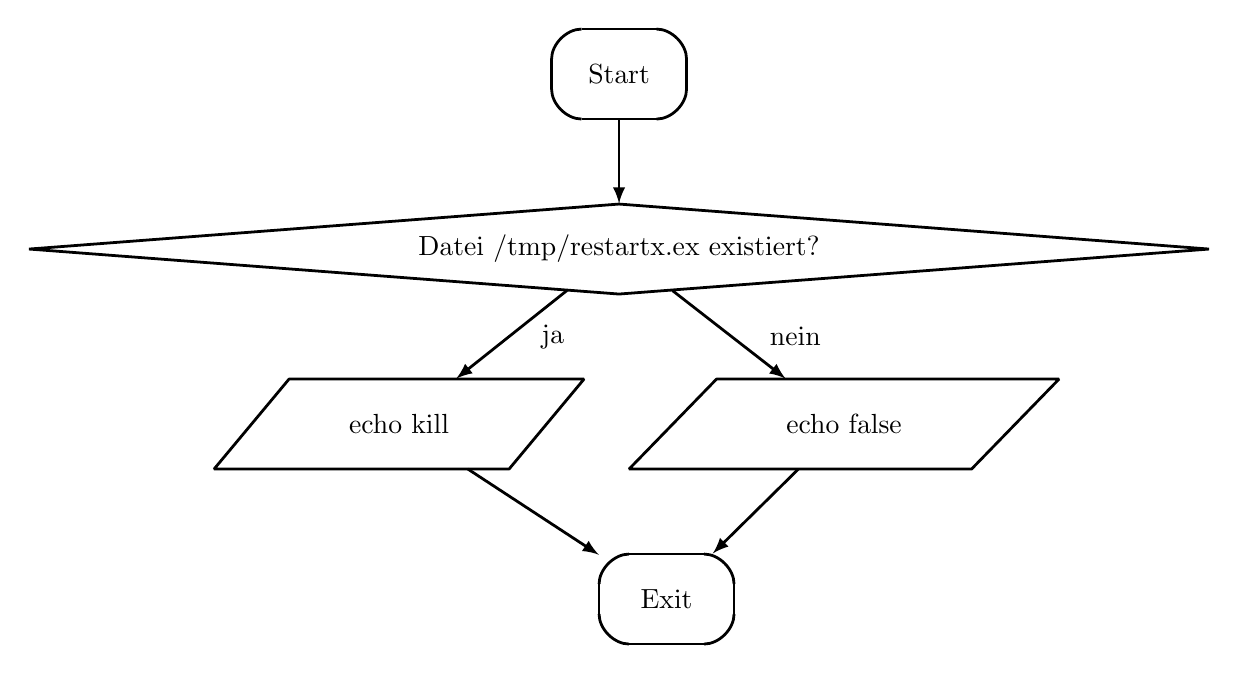
\begin{tikzpicture}[>=latex,line join=bevel,scale=0.9]
  \pgfsetlinewidth{1bp}
%%
\pgfsetcolor{black}
  % Edge: Start -> Datei /tmp/restartx.ex existiert?
  \draw [->] (236bp,209.97bp) .. controls (236bp,202.76bp) and (236bp,194.28bp)  .. (236bp,176.21bp);
  % Edge: Datei /tmp/restartx.ex existiert? -> echo false
  \draw [->] (257.33bp,141.41bp) .. controls (268.39bp,132.8bp) and (282.13bp,122.12bp)  .. (302.61bp,106.19bp);
  \definecolor{strokecol}{rgb}{0.0,0.0,0.0};
  \pgfsetstrokecolor{strokecol}
  \draw (306.5bp,123bp) node {nein};
  % Edge: echo false -> Exit
  \draw [->] (307.72bp,69.973bp) .. controls (299.5bp,61.872bp) and (289.66bp,52.169bp)  .. (273.47bp,36.209bp);
  % Edge: Datei /tmp/restartx.ex existiert? -> echo kill
  \draw [->] (215.15bp,141.41bp) .. controls (204.33bp,132.8bp) and (190.9bp,122.12bp)  .. (170.87bp,106.19bp);
  \draw (209.5bp,123bp) node {ja};
  % Edge: echo kill -> Exit
  \draw [->] (175.56bp,69.973bp) .. controls (188.89bp,61.251bp) and (205.06bp,50.674bp)  .. (227.91bp,35.723bp);
  % Node: echo kill
\begin{scope}
  \definecolor{strokecol}{rgb}{0.0,0.0,0.0};
  \pgfsetstrokecolor{strokecol}
  \draw (222bp,106bp) -- (104bp,106bp) -- (74bp,70bp) -- (192bp,70bp) -- cycle;
  \draw (148bp,88bp) node {echo kill};
\end{scope}
  % Node: Start
\begin{scope}
  \definecolor{strokecol}{rgb}{0.0,0.0,0.0};
  \pgfsetstrokecolor{strokecol}
  \draw (251bp,246bp) -- (221bp,246bp);
  \draw (221bp,246bp) .. controls (215bp,246bp) and (209bp,240bp)  .. (209bp,234bp);
  \draw (209bp,234bp) -- (209bp,222bp);
  \draw (209bp,222bp) .. controls (209bp,216bp) and (215bp,210bp)  .. (221bp,210bp);
  \draw (221bp,210bp) -- (251bp,210bp);
  \draw (251bp,210bp) .. controls (257bp,210bp) and (263bp,216bp)  .. (263bp,222bp);
  \draw (263bp,222bp) -- (263bp,234bp);
  \draw (263bp,234bp) .. controls (263bp,240bp) and (257bp,246bp)  .. (251bp,246bp);
  \draw (236bp,228bp) node {Start};
\end{scope}
  % Node: Exit
\begin{scope}
  \definecolor{strokecol}{rgb}{0.0,0.0,0.0};
  \pgfsetstrokecolor{strokecol}
  \draw (270bp,36bp) -- (240bp,36bp);
  \draw (240bp,36bp) .. controls (234bp,36bp) and (228bp,30bp)  .. (228bp,24bp);
  \draw (228bp,24bp) -- (228bp,12bp);
  \draw (228bp,12bp) .. controls (228bp,6bp) and (234bp,0bp)  .. (240bp,0bp);
  \draw (240bp,0bp) -- (270bp,0bp);
  \draw (270bp,0bp) .. controls (276bp,0bp) and (282bp,6bp)  .. (282bp,12bp);
  \draw (282bp,12bp) -- (282bp,24bp);
  \draw (282bp,24bp) .. controls (282bp,30bp) and (276bp,36bp)  .. (270bp,36bp);
  \draw (255bp,18bp) node {Exit};
\end{scope}
  % Node: Datei /tmp/restartx.ex existiert?
\begin{scope}
  \definecolor{strokecol}{rgb}{0.0,0.0,0.0};
  \pgfsetstrokecolor{strokecol}
  \draw (236bp,176bp) -- (0bp,158bp) -- (236bp,140bp) -- (472bp,158bp) -- cycle;
  \draw (236bp,158bp) node {Datei /tmp/restartx.ex existiert?};
\end{scope}
  % Node: echo false
\begin{scope}
  \definecolor{strokecol}{rgb}{0.0,0.0,0.0};
  \pgfsetstrokecolor{strokecol}
  \draw (412bp,106bp) -- (275bp,106bp) -- (240bp,70bp) -- (377bp,70bp) -- cycle;
  \draw (326bp,88bp) node {echo false};
\end{scope}
%
\end{tikzpicture}

